% Drawing 142/02-4 -- folder 142, batch 02, archive page 27 (PDF page 28).
% Transcription: à gauche : sphère portant les trois sommets $Q_0$, $Q_1$, $Q_\infty$ et les six arcs $\tilde a_i^{\pm}$ qui les joignent deux à deux. Légende : $\mathrm{III}_J$.
% Kind: sphere with three vertices and six arcs. Method 2 (schematic redraw from the facsimile). Status: partial.
% Notes: Sphere in pencil; Q_1 (left), Q_infty (middle), Q_0 (right) on the front, joined pairwise by two arcs each: a lens Q_1-Q_infty, a lens Q_infty-Q_0, and an arc Q_1-Q_0 over the top (dotted); the sixth arc (tilde a_infty^-, Q_1-Q_0) is drawn by him across the middle, overinked. Arrowheads are approximate. Legend III_J and (27) are text.
% Coordinates: 1 unit = 1 mm = 1/100 of the crop width (bbox in page fractions: [0.15, 0.42, 0.38, 0.54]).
% Redrawn by Claude (claude-opus-5-5), issue #73, 2026-11-07; not checked by a human; not compiled (no TeX in the session).
% Rights: reproduces part of the work -- behind RENDER_TRANSCRIPTS, never published by itself.
\documentclass[tikz,border=3pt]{standalone}
\usepackage{amsmath,amssymb}
\usetikzlibrary{patterns,arrows.meta}
\tikzset{pencil/.style={black!45}, struck/.style={black!35}, mark/.style={circle,draw,inner sep=1.3pt}, pt/.style={circle,fill,inner sep=0.9pt}, opt/.style={circle,draw,fill=white,inner sep=1.1pt}}
\begin{document}
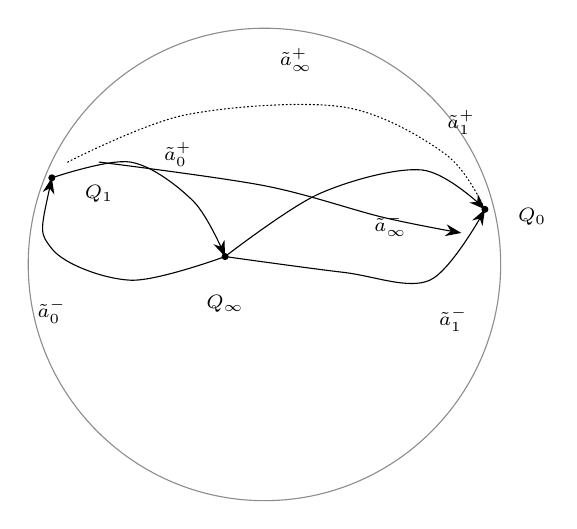
\begin{tikzpicture}[x=1mm,y=1mm,line cap=round,line join=round,font=\scriptsize]
\draw[pencil] (35,-40) circle[radius=30];
\node[pt] at (8,-29) {};
\node[pt] at (30,-39) {};
\node[pt] at (63,-33) {};
\draw[-{Stealth[length=2mm]}] plot[smooth, tension=0.55] coordinates {(8,-29) (18,-27) (26,-32) (30,-39)};
\draw[{Stealth[length=2mm]}-] plot[smooth, tension=0.55] coordinates {(8,-29) (8,-38) (18,-42) (30,-39)};
\draw[-{Stealth[length=2mm]}] plot[smooth, tension=0.55] coordinates {(30,-39) (42,-31) (55,-28) (63,-33)};
\draw[-{Stealth[length=2mm]}] plot[smooth, tension=0.55] coordinates {(30,-39) (45,-41) (56,-42) (63,-33)};
\draw[densely dotted] plot[smooth, tension=0.55] coordinates {(10,-27) (25,-21) (45,-20) (58,-26) (63,-33)};
\draw[-{Stealth[length=2mm]}] plot[smooth, tension=0.55] coordinates {(14,-27) (35,-30) (50,-34) (60,-36)};
\node[inner sep=1pt] at (14,-31) {\scriptsize $Q_1$};
\node[inner sep=1pt] at (30,-45) {\scriptsize $Q_\infty$};
\node[inner sep=1pt] at (69,-34) {\scriptsize $Q_0$};
\node[inner sep=1pt] at (39,-14) {\scriptsize $\tilde a_\infty^{+}$};
\node[inner sep=1pt] at (24,-26) {\scriptsize $\tilde a_0^{+}$};
\node[inner sep=1pt] at (60,-22) {\scriptsize $\tilde a_1^{+}$};
\node[inner sep=1pt] at (8,-46) {\scriptsize $\tilde a_0^{-}$};
\node[inner sep=1pt] at (51,-35) {\scriptsize $\tilde a_\infty^{-}$};
\node[inner sep=1pt] at (59,-47) {\scriptsize $\tilde a_1^{-}$};
\end{tikzpicture}
\end{document}
